\chapter{Probleme}

\section{Cuplaj cu costuri pe noduri}

\noindent \textbf{Enunț.} Se dă un graf bipartit $G(U + V, E)$ și o funcție de cost $w \colon U \to \mathbb{R}$. Să se determine cuplajul
maximal care maximizează suma costurilor nodurilor alese în cuplaj.

\noindent \textbf{Soluție.} Este corect să prioritizam nodurile în ordinea descrescătoare a costurilor asociate.

\begin{lem}
  \textbf{Berge}. Un cuplaj $M$ în $G$ este maximal dacă și numai dacă nu există o cale care pornește dintr-un nod nesaturat, se încheie pe un alt
  nod nesaturat și alternează între muchii alese în $M$ și restul.
\end{lem}

\begin{proof}
  Să presupunem că executând algoritmul în ordinea sortată obținem cuplajul $A$, iar cel optim este de fapt $B$.
  Fie $u$ primul nod în ordinea descrescătoare a costurilor care nu este saturat în $B$, dar este saturat în $A$.
  Pentru că $u$ a fost cuplat înaintea nodurilor cu cost mai mic decât el, atunci exista un lanț alternant în
  $A \oplus B$ de la $u$ către un alt nod din $U$, $u'$, pentru care $w(u) \geq w(u')$. Acest lanț ar putea fi folosit
  în $B$ și ar aduce un cost total cel puțin la fel de bun.
\end{proof}

O explicație alternativa, relevantă problemelor de optimizare este teoria despre matroizi \cite{matroid}. Un matroid $M$ este o pereche
$(E, I)$, unde $E$ este o mulțime, iar $I$ este o familie de submulțimi ale lui $E$, iar cele două satisfac următoarele condiții:

\begin{itemize}
  \item Mulțimea $E$ este finită.
  \item Familia $I$ este ereditară, mai exact $s \in I, s' \subset s \implies s' \in I$.
  \item Pentru doua submulțimi $s_{1}, s_{2} \in I$, cu $|s_{1}| < |s_{2}|$, există un element
    $x \in s_{2} - s_{1}$ astfel încât $s_{1} \cup \{x\} \in I$.
\end{itemize}

Elementele lui $I$ se numesc submulțimi independente. Dacă se poate asocia o greutate fiecărei submulțimi independente, atunci un rezultat
important al acestei structuri este că, pentru a găsi submulțimea independentă de cost maxim, este de ajuns să construim un algoritm greedy
care pornește cu submulțimea vidă (care prin definiție face parte din $I$) și încearcă să adauge pe rând elemente din $M$, în ordinea descrescătoare
a costurilor.

Problema cuplajului maximal este de fapt o intersecție de matroizi. Unul din aceștia este matroidul $(U, I)$, unde $I$ sunt submulțimi de noduri
din $U$, pentru care există cel puțin un cuplaj în care toate nodurile din submulțime sunt saturate. Greutatea unei submulțimi este suma valorilor
imaginii funcției $w$ peste această submulțime. Rămâne să verificam că este într-adevăr un matroid:

\begin{itemize}
  \item Mulțimea $U$ este finită.
  \item Daca știm un cuplaj pentru o mulțime de noduri, atunci putem construi cuplajul pentru orice submulțime, păstrând doar perechile nodurilor
  rămase.
  \item Reamintim că matroidul este pe noduri din $U$, nu pe perechi de noduri cuplate. Fie $M_{1}$ și $M_{2}$ doua submulțimi independente pentru care
    $|M_{2}| \geq |M_{1}|$, atunci din reciproca \textbf{lemei lui Berge}, putem mări cuplajul $M_{1}$ folosind un nod din $M_{2} - M_{1}$ păstrând
    toate nodurile din $M_{1}$.
\end{itemize}

Apoi, se poate observa că Eliminarea Gaussiana (\ref{gauss}) se poate comporta greedy în căutarea rangului, deoarece poate prioritiza în timpul pivotării
acele linii (asociate nodurilor) în ordinea descrescătoare a valorii funcției $w$.

\pagebreak

\section{Cuplaj cu costuri pe muchii}

\noindent \textbf{Enunț.} Se dă un graf bipartit $G(U + V, E)$ și o funcție de cost $w \colon E \to \mathbb{R}$. Să se determine cuplajul
\textbf{perfect} care maximizează suma costurilor muchiilor alese în cuplaj.

\noindent \textbf{Soluție.} Considerăm următoarea formulare a problemei ca una de programare liniară (\cite{assignmentlp}):

\begin{equation*}
\begin{array}{ll@{}ll}
  \text{max}  & \displaystyle\sum\limits_{(x, y) \in E} w((x, y))m_{x, y} &\\
  \text{s.t.} & \displaystyle\sum\limits_{y} m_{x, y} = 1 \ \forall \ x &\\
              & \displaystyle\sum\limits_{x} m_{x, y} = 1 \ \forall \ y &\\
              & m_{x,y} \in \{0, 1\} \ \forall x, y
\end{array}
\end{equation*}

Aceasta este o problema discreta pentru că am condiționat ca $m_{x, y}$ să fie $0$ sau $1$, dar se poate arata că în cazul problemei cuplajului
de cost maxim putem relaxa aceasta condiție la varianta continua și anume $0 \leq m_{x, y} \leq 1$. \textbf{Teorema Birkhoff-von Neumann} spune
că fiecare cuplaj fracționar poate fi descompus ca o combinație convexa de cuplaje. Să considerăm formularea duala a acestei probleme:

\begin{equation*}
\begin{array}{ll@{}ll}
  \text{min}  & \displaystyle\sum\limits_{x} p_{x} + \displaystyle\sum\limits_{y} q_{y} &\\
  \text{s.t.} & p_{x} + q_{y} \leq w((x, y)) \ \forall \ (x, y) \in E &\\
              & \displaystyle\sum\limits_{y} q_{y} m_{x, y} = q_{y} \ \forall \ x &\\
              & \displaystyle\sum\limits_{x} p_{x} m_{x, y} = p_{x} \ \forall \ y &\\
\end{array}
\end{equation*}

Duala unei probleme de maximizare este una de minimizare, iar optimul ei consistuie o limita superioară pentru problema primala
\textbf{(dualitate ușoară)}. Atunci când este chiar egala, se numește \textbf{dualitate puternică}.

\begin{thm}
  Problema cuplajului perfect de cost maxim admite dualitate puternică.
\end{thm}

\begin{thm}
  Duala problemei cuplajului maximal este acoperirea muchiilor cu număr minim de noduri.
\end{thm}

\begin{proof}
  Daca am formula problema cuplajului maximal ca o problema de programare liniară atunci golul ar fi să maximizăm numărul de muchii alese,
  cu restricția că fiecare nod trebuie să aibă cel mult o muchia aleasă incidenta. Folosind iar \textbf{teorema Birkhoff-von Neumann} putem
  arata că putem relaxa problema dintr-una discretă într-una continuă. Duala acestei probleme este să se minimizeze numărul de noduri alese
  cu restricția că fiecare muchie trebuie să aibă măcar un nod ales. Aceasta este chiar problema acoperirii muchiilor cu număr minim de noduri.
\end{proof}

\textbf{Algoritmul ungar} este un algoritm care rezolvă problema cuplajului de cost maxim, folosindu-se de dualitatea prezentată. Acesta
construiește simultan un cuplaj perfect de cost minim și soluția duala a căror valoare este egală cu costul cuplajului. Se păstrează
următorii invarianți:

\begin{itemize}
  \item Fiecare muchie $(x, y)$ satisface $p_{x} + q_{y} \geq w((x, y))$. Dacă $p_{x} + q_{y} = w((x, y))$, atunci $(x, y)$ este o muchie strânsă.
  \item Muchiile alese în cuplaj sunt și strânse.
  \item După fiecare faza a algoritmului, mărimea cuplajului creste cu $1$ până ajunge la cel perfect.
\end{itemize}

\noindent Algoritmul urmărește acești pasi (\cite{hungarian}):

\begin{enumerate}
  \item Initializam $p_{x} = 0 \ \forall \ x$ și $q_{y} = \max w((x, y)) \ \forall \ (x, y) \in E \ \forall \ y$.
  \item Se caută cuplajul maximal folosind doar muchii strânse.
  \item Dacă cuplajul este perfect algoritmul se termină. Altfel, folosind cuplajul calculat, se calculează dualul $C$,
    adică acoperirea muchiilor cu număr minim de noduri.
  \item Se calculează $\bigtriangleup = \text{min}_{(x, y) \in E, x \notin C, y \notin C} p_{x} + q_{y} - w((x, y))$.
  \item Potențialii se recalculează după urmatorea regula:
    \begin{itemize}
      \item $p_{x} = p_{x} + \bigtriangleup \ \forall \ x \in C$
      \item $q_{y} = q_{y} - \bigtriangleup \ \forall \ y \notin C$
    \end{itemize}
  \item Repetă pasul 2.
\end{enumerate}

Se observă că algoritmul ungar folosește algoritmul de cuplaj maximal ca un oracol. În lucrarea inițială se folosește un algoritm bazat pe
ideea de la algoritmii de flux maxim, incrementand dimensiunea cuplajului mereu cu 1, găsind o cale alternanta $P$ și înlocuind cuplajul $M$
cu $M \oplus P$. Însă aici putem folosi metodele algebrice studiate.

Pentru a calcula cuplajul maximal este de ajuns să găsim rangul matricei Edmonds asociată grafului, adică mărimea bazei formată din spațiul
liniar al vectorilor de pe linii. Acestea vor fi chiar nodurile alese în cuplaj din $U$.

Ce rămâne de făcut este având cuplajul $M$, să găsim acoperirea muchiilor cu număr minim de noduri $C$. $C$ se poate construi alegând
câte un nod din fiecare muchie din $M$. Pentru fiecare muchie $i$ din cuplaj putem crea un literal $x_{i}$ care să fie adevărat daca alegem
nodul din mulțimea $V$ și fals dacă alegem nodul din mulțimea $U$. Relațiile intre aceștia se pot scrie că o formulă 2-CNF. Considerăm o
muchie $(u,v) \in E - M$, atunci:
\begin{itemize}
  \item Dacă $u$ și $v$ sunt noduri saturate, atunci fie $i_{1}$, respectiv $i_{2}$ muchiile din cuplaj asociate. În acest caz adaugăm clauza
  $\neg x_{i_{1}} \lor x_{i_{2}}$, însemnând că fie $i_{1}$ își folosește capătul din $U$, fie $i_{2}$ își folosește capătul din $V$.
  \item Dacă $u$ este saturat, iar $v$ nu, atunci fie $i$ muchia din cuplaj asociată. Trebuie ca $u$ să fie inclus în $C$, deci $x_{i}$ trebuie
  să fie fals.
  \item Aidoma dacă $v$ este saturat, iar $u$ nu.
  \item Ambele noduri nu pot să fie nesaturate, pentru că ar contrazice faptul că $M$ este un cuplaj maximal.
\end{itemize}

Presupunem că $|U|, |V| = O(n)$. Problema de 2-SAT se poate rezolva apoi în complexitate de timp $O(n^{2})$. Acest proces se poate simplifica
în implementare pentru că în $C$ vor fi chiar acele noduri aflate la distanță impară de nodurile nesaturate din $U$.

În acest algoritm mărimea cuplajului nu vă scădea niciodată, iar aceasta creste până la $|U|$. De fiecare data când se schimba
mărimea cuplajului, putem să recalculam mulțimea muchiilor și acoperirea minima în timp $O(n^{3})$. Până să crească mărimea
cuplajului pot exista $O(n)$ schimbări de potențiale. Putem să determinam în timp $O(n^{2})$ pentru fiecare dintr-acestea
cum modifică rangul. În total algoritmul are complexitate de timp $O(n^{4})$, dar folosește primitive algebrice care se pot
executa în paralel sau chiar concurent pe procesoarele moderne și pot beneficia de toate optimizările cunoscute, printre care
și algoritmul lui Coppersmith (\ref{coppersmith}).

\section{Izomorfism de subarbori}
\begin{tabular}{l@{\extracolsep{1cm}}l}
  Concurs: & Lot Informatică Râmnicu Vâlcea 2015 - Baraj 2 Seniori\\
  Limita de timp: & 0.3\ s\\
  Limita de memorie: & 64\ MB\\
\end{tabular}

\hspace{1cm}

\noindent \textbf{Enunț.} Se dau doi arbori cu rădăcină în nodul $0$ și cel mult $500$ de noduri, $A$ și $B$.
O operație constă în ștergerea unei frunze. Care este numărul minim de operații aplicate pe $A$ astfel încât
să devină izomorf cu $B$?

\noindent \textbf{Soluție.} Cei doi arbori sunt izomorfi dacă există o re-etichetare a nodurilor în așa fel încât să fie identici.
Considerăm mai întăi o problema mai simplă: cum vedem dacă doi arbori sunt izomorfi? Vom atribui fiecărui arbore un polinom în mai
multe variabile și vom reduce problema la una de echivalență de polinoame.

\begin{figure}[H]
  \centering
  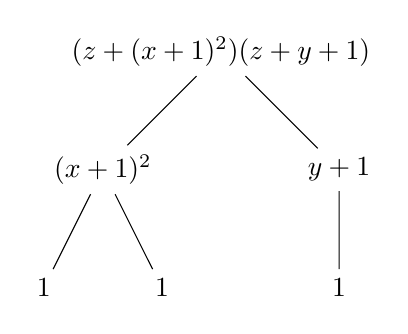
\begin{tikzpicture}[level distance=1.5cm,
    level 1/.style={sibling distance=3cm},
    level 2/.style={sibling distance=1.5cm}]
    \node {$(z + (x + 1)^{2})(z + y + 1)$}
      child {node {$(x + 1)^{2}$}
        child {node {$1$}}
        child {node {$1$}}
      }
      child {node {$y + 1$}
      child {node {$1$}}
      };
  \end{tikzpicture}
  \caption{Construcția polinomului}
\end{figure}

\begin{algorithm}[H]
  \DontPrintSemicolon
  \SetKwFunction{FMain}{DFS-POLY}
  \SetKwProg{Fn}{Function}{:}{}
  \Fn{\FMain{$T$, $u$, $p$}}{
    poly := 1\;
    \For{$v \in T_{u}$}{
      \If{$v \neq p$}{
        poly := poly * ($x_{u}$ + DFS-POLY(T, v, u))\;
      }
    }
    \KwRet poly\;
  }
  \;
\end{algorithm}

Pentru doi arbori, dacă evaluăm polinoamele cu valori uniform aleatoare alese din $\mathbb{F}_{p}$, atunci probabilitatea de coliziune este de
cel mult $\frac{N}{p}$, unde $N$ este numărul de noduri, conform lemei \textbf{Schwartz-Zippel}. Doi arbori ne-izomorfi vor avea polinoamele diferite
pentru ca inelul polinoamelor $\mathbb{F}_{p}[x_{1}, x_{2}, \ldots, x_{N}]$ determină o factorizare unică a polinomului, descompus într-un produs de
polinoamele ireductibile și constante.

Având acest algoritm, putem construi o soluție cu backtracking în care pornind din frunze, eliminăm o mulțime de noduri, mai exact atâtea
noduri cât are $A$ în plus fata de $B$ și apoi verificăm izomorfismul cu algoritmul dat.

În continuare, observam din soluția precedenta că răspunsul este fix $|A| - |B|$, daca exista o secvență de operații. Vom nota cu $a_{v_{1}}$
subarborele nodului $v_{1}$ din $A$ și cu $b_{v_{2}}$ subarborele nodului $v_{2}$ din $B$. Vom construi următoarea recurență folosind
programare dinamică: $d_{v_{1}, v_{2}}$ este adevărat dacă putem executa o secvență de operații astfel încât să transformăm subarborele
nodului $v_{1}$ într-unul izomorfm subarborelui nodului $v_{2}$ (din celalalt arbore). Este clar că pentru perechi unde $|a_{v_{1}}| < |b_{v_{2}}|$ valoarea va fi fals. Altfel, considerăm fii direcți ai acestor două noduri: $c_{1, 1}, c_{1, 2}, \ldots, c_{1, n_{1}}$ și $c_{2, 1}, c_{2, 2}, \ldots, c_{2, n_{2}}$.
Dacă $n_{1} < n_{2}$, atunci nu se poate să eliminăm noduri, micșorând astfel $n_{1}$, încât să obținem $n_{2}$. În ce urmează ne interesează să găsim o
submulțime a fiilor primului nod $c_{1, i_{1}}, c_{1, i_{2}}, \ldots, c_{1, i_{n_{2}}}$ astfel încât $d_{c_{1, i_{j}}, c_{2, j}}$ să fie adevărate
pentru toți $1 \leq j \leq n_{2}$.

O primă soluție ar fi să considerăm toate cele $\binom{n_{1}}{n_{2}}$ soluții posibile. Aceasta soluție este deja mai eficientă decât prima propusă.

\begin{thm}
  \label{hall}
  \textbf{Hall.} Fie $G = (U \cup V, E)$ un graf bipartit. Există un cuplaj care acoperă $U$ dacă și numai dacă pentru orice submulțime $W$
  a lui $U$, dacă am considera mulțimea $N_{G}(W)$ ca fiind reuniunea vecinilor nodurilor din $W$, atunci $|W| \leq N_{G}(W)$.
\end{thm}

Cum putem folosi \textbf{teorema lui Hall} în cazul nostru este să construim matricea $d'$ asociată vecinilor lui $v_{1}$, respectiv $v_{2}$
unde $d'_{i, j} = d_{c_{1, i}, c_{2, j}}$. Dacă pentru fiecare mulțime de coloane considerăm mulțimea liniilor care au măcar o valoare de adevărat
pe vreuna din coloane, atunci vrem ca numărul de linii să nu fie mai mic decât numărul de coloane. Această soluție din păcate rămâne exponențială
și se poate construi în timp $O(2^{n_{2}} n_{1})$ daca se procesează submulțimile de coloane în ordinea codurilor Gray, în timp ce soluția evidentă ar lua
$O(2^{n_{2}} n_{1}n_{2})$. O proprietate inedită a codurilor Gray este că măștile consecutive de biți vor fi diferite pe fix un bit. Astfel vom determina acel bit,
asociat unei coloane și apoi vom folosi un vector de frecvență pentru a determina ce linii mai rămân active pentru noua submulțime de coloane, în timp
cel mult $O(n_{1})$.

Problema pe matricea $d'$ este chiar de cuplaj în graf bipartit, iar $d'$ este chiar textbf{matricea Edmonds} (\ref{edmonds}). Rămâne să îi calculam
rangul și să verificăm că este egal cu $n_{2}$. Complexitatea acestei soluții este:

\begin{equation}
  \displaystyle\sum\limits_{v_{1} \in A} \displaystyle\sum\limits_{v_{2} \in B} n_{1}n_{2}^{2} = \displaystyle\sum\limits_{v_{1} \in A} n_{1} \displaystyle\sum\limits_{v_{2} \in B} n_{2}^{2} \leq |A||B|^{2}
\end{equation}

\noindent pentru că $a^{2} + b^{2} \leq (a + b)^{2}$.

\pagebreak

\section{Acoperire cu cai a unui graf orientat aciclic}

\noindent \textbf{Enunt.} Se da un graf orientat aciclic $G(V, E)$. Sa se gaseasca o multime de cardinal minim de cai, astfel incat
fiecare nod sa faca parte din exact o cale.

\noindent \textbf{Solutie.} Un graf orientat aciclic este un graf orientat fara cicli orientati. Acesta admite o sortate topologica,
adica o ordonare a nodurilor $v_{1}, v_{2}, \ldots$ in asa fel incat daca exista arcul $(v_{i}, v_{j})$, atunci $v_{i}$ apare inaintea
lui $v_{j}$ in ordonare. Algoritmul pentru a calcula sortarea topologica este urmatorul:

\begin{algorithm}[H]
  \DontPrintSemicolon
  \SetKwFunction{FMain}{DFS-VISIT}
  \SetKwProg{Fn}{Function}{:}{}
  \Fn{\FMain{$G$, $color$, $u$, $T$}}{
    \If{$color_{u}$ = BLACK}{
      \KwRet T\;
    }
    $color_{u}$ := GRAY\;
    \For{$v \in G_{u}$}{
      T := DFS-VISIT($G, color, v, T$)\;
    }
    $color_{u}$ := BLACK\;
    \KwRet [u] + T\;
  }
  \;
\end{algorithm}

\begin{algorithm}[H]
  \DontPrintSemicolon
  \SetKwFunction{FMain}{DFS}
  \SetKwProg{Fn}{Function}{:}{}
  \Fn{\FMain{$G$}}{
    \For{$u \in G$}{
      $color_{u}$ := WHITE\;
    }
    T := []\;
    \For{$u \in G$}{
      T := DFS-VISIT(G, color, u, T)\;
    }
    \KwRet T\;
  }
  \;
\end{algorithm}

\pagebreak

Algoritmul practic construiește inversa postordinii și aceasta este chiar o sortare topologică posibila.

Având calculată sortarea topologică, o prima soluție cu backtracking vă considera nodurile în ordinea inversă.
Ne putem imagina căile ca o colorare, iar acum la fiecare pas al algoritmului trebuie să stabilim culoarea pentru
nodul curent. Pentru că le procesam în ordinea inversa sortării topologice, știm că am procesat deja toți vecinii lui
iar aceștia sunt colorați în culorile $\{C_{1}, C_{2}, \ldots, C_{k}\}$. Pentru a asigura invariantul de cale, odată ce
un nod preia culoarea unui vecin, vecinul își pierde culoarea și nu mai poate fi ales pe măsură ce coborâm în adâncime.
Atunci, pentru nodul curent trebuie să alegem una din aceste culori sau să creăm o culoare nouă. După ce toate nodurile
au fost colorate putem să ne uităm la numărul de culori diferite folosite și aceasta vă fi un candidat pentru răspunsul
problemei.

\begin{lem}
  Complexitatea acestei soluții este de $O(|E|2^{|V|})$.
\end{lem}

\begin{proof}
  În cel mai rău caz, considerăm nodurile în ordine și la fiecare pas avem o decizie, ne atașam la o cale existentă sau creăm o cale
  nouă.
\end{proof}

\noindent Soluția polinomială a problemei nu este evidentă, dar este sugerată de conexiunea cuplajului în graf bipartit cu teorema lui
Dilworth. Vom numi o \textbf{anticale} o secvență de noduri $v_{1}, v_{2}, \ldots, v_{k}$ pentru care
$\forall \ v_{i}, v_{j} \ (v_{i}, v_{j}), (v_{j}, v_{i}) \notin E$.

\begin{thm}
  \label{Dilworth}
  \textbf{Dilworth.} Numărul minim de cai necesare ca să acoperi graful este egal cu mărimea celei mai lungi anticai.
\end{thm}

\begin{thm}
  \label{Konig}
  \textbf{Kőnig (1931).} În orice graf bipartit, numărul de muchii dintr-un cuplaj maximal este egal cu numărul de noduri din acoperirea minimă.
\end{thm}

Având această observație, este mai clară reducerea la cuplaj în graf bipartit. Construim graful bipartit în care dublăm fiecare nod din graful
inițial astfel încât să apară în ambele mulțimi. Apoi, muchiile din graful inițial le vom considera și în acesta, doar că vor conecta doar
noduri din mulțimi diferite. Acum, dacă am găsi o mulțime maximă de noduri independente, aceasta va fi o \textbf{anticale}.

\pagebreak

\section{Bilingual}

\begin{tabular}{l@{\extracolsep{1cm}}l}
  Concurs: & Google Code Jam 2015 Round 2\\
  Limita de timp: & 10\ s\\
  Limita de memorie: & 256\ MB\\
\end{tabular}

\hspace{1cm}

\noindent \textbf{Enunț.} Se dau $N + 2 \ (2 \leq N \leq 200)$ liste de cuvinte. Se știe că prima listă conține doar cuvinte în limba
engleza, a doua conține doar cuvinte în limba franceză. Restul de $N$ nu se cunosc și trebuie catalogate într-una
din cele două limbi în așa fel încât să se minimizeze numărul de cuvinte care fac parte din ambele limbi.

\hspace{1cm}

\noindent \textbf{Soluție.} O prima soluție cu backtracking trebuie să asocieze fiecărei liste o limbă și apoi să
verifice numărul de cuvinte care se află în ambele limbi. Sunt $2^{N}$ posibilități de a alege, iar verificarea poate
dura și până la suma numărului de cuvinte, dacă acestea se normalizează în prealabil. Sunt mai multe moduri în care
putem îmbunătăți constanta acestei soluții. În primul rand, putem ignora cuvintele care nu apar în mai mult de o
propoziție. De asemenea, în cazul acestui backtracking, o alta optimizare semnificativa ar fi iterative deepening pe răspuns,
adică să nu urmărim ramuri care cresc numărul de cuvinte incompatibile din răspuns imediat ce le observăm (depth-first),
dar să o abordam gradual și să preferam o creștere în lățime, nu în adâncime. Din păcate aceasta soluție nu este destul
de rapidă, nici măcar pentru anul $2015$, când soluțiile la Code Jam se rulau local și se cerea doar rezultatul unei
rulări de program.

Problema se aseamănă unei probleme clasice de tăietură minimă, numită \textbf{Image segmentation}. Tăietură minimă este duala
problemei de flux maxim. În aceasta problemă sunt $N$ pixeli. Fiecărui pixel $i$ se poate asocia o culoare de prim plan de cost
$f_{i}$ sau o culoare de fundal $b_{i}$. Dacă doi pixeli $i$ și $j$ sunt adiacenți și au asocieri diferite, atunci trebuie scăzută
o valoare $p_{i,j}$. Problema cere să se efectueze asocierile în așa fel încât să maximizeze costul. Fie $P$ mulțimea pixelilor cărora
le-a fost asociat prim-planul și $Q$ mulțimea pixelilor cărora le-a fost asociat fundalul, atunci dorim să maximizăm
$\displaystyle\sum\limits_{i \in P} f_{i} + \displaystyle\sum\limits_{i \in Q} b_{i} - \displaystyle\sum\limits_{i \in P, j \in Q \lor i \in Q, j \in P} p_{i,j}$. Aceasta se poate reformula ca o problemă
de minimizare a valorii $\displaystyle\sum\limits_{i \in P, j \in Q \lor i \in Q, j \in P} p_{i,j}$. Rețeaua de flux maxim dublează nodurile pentru fiecare pixel
în așa fel încât un nodul $2u$ înseamnă $u$ a fost asociat pe prim-plan, iar $2u+1$ înseamnă $u$ a fost asociat pe fundal. Sursa este
conectată către toate nodurile de prim-plan $2u$ cu capacitate $f_{u}$, iar destinația este conectată către toate nodurile de fundal $2u+1$
cu capacitate $b_{u}$. Muchii de capacitate $p_{i,j}$ se adaugă între nodurile adiacente de asocieri diferite. O tăietură de la sursa la
destinație este apoi o asociere a pixelilor în mulțimile $P$, respectiv $Q$.

În cazul nostru, culoarea de prim plan înseamnă un cuvânt în limba engleză, iar culoarea de fundal înseamnă un cuvânt în limba franceză.
Observăm că nu ne interesează valorile $f_{i}, b_{i}$, trebuie doar să fie suficent de mari, iar valoarea de ``penalty'' se aplică atunci când
un cuvânt este asociat în ambele limbi și are cost $1$. Trebuie totuși să avem grija să nu atribuim mai multe limbi aceleiași liste, așadar mai
asociem un cost $\inf$ între cuvinte de limbă diferită din aceeași propoziție. Trebuie tratate cu atenție cuvintele din primele două propoziții.

În schimb, nu am prezentat degeaba această problemă. Ea poate fi rezolvată mai departe și ca o problema de cuplaj maxim în graf bipartit.
Putem împarți cuvintele în trei mulțimi, cuvintele care sunt doar în engleză, cuvintele care sunt doar în franceză și cuvintele
care sunt în ambele limbi. Pentru a minimiza numărul de cuvinte din ambele limbi ne dorim să maximizăm numărul de cuvinte care sunt într-o
singură limba. Ca înainte, vom construi două noduri pentru fiecare cuvânt $u$, nodul $2u$ va fi ales dacă $u$ nu este un cuvânt în engleză,
iar nodul $2u + 1$ vă fi ales dacă $u$ nu este un cuvânt în franceză. Pentru fiecare două cuvinte $u_{1}, u_{2}$ din aceeași lista adaugăm o
muchie între $2u_{1}$ și $2u_{2} + 1$. Rămâne de găsit cea mai mare mulțime de noduri astfel încât nu există o muchie între nicio pereche, adică
\textbf{maximal independent set}. Pe caz general aceasta nu se poate rezolva polinomial, însă graful creat este evident unul bipartit. În grafurile
bipartite \textbf{maximal independent set} este complementul acoperirii minime cu nodurilor (\textbf{minimal vertex cover}).

Așadar, folosind \ref{Konig}, putem folosi algoritmul de cuplaj maximal \ref{Algoritm paralelizabil pentru cuplaj} pentru a calcula răspunsul problemei.

\pagebreak

\section{Paritatea numărului de cuplaje}
\begin{tabular}{l@{\extracolsep{1cm}}l}
  Concurs: & Olimpiada națională pentru studenți 2015, Runda finală\\
  Limita de timp: & 1\ s\\
  Limita de memorie: & 20\ MB\\
\end{tabular}

\hspace{1cm}

\noindent \textbf{Enunț.} Se dă un graf bipartit $G = (U + V, E)$ unde $|U|, |V| \leq 100$. Să se determine paritatea numărul de cuplaje perfecte.

\hspace{1cm}

\noindent \textbf{Soluție.} Este clar că dacă $|U| \neq |V|$ atunci numărul este $0$, deci par. Altfel, putem pentru început să testăm fiecare permutare, în complexitate $O(|U|!)$.

Putem îmbunătăți soluția precedenta dacă o abordăm cu programare dinamică. Construim tabela $D_{i, S}$ care este paritatea numărului de cuplaje a
primelor $i$ elemente din $U$ cu mulțimea de noduri din $S \subseteq V$. Recurența se poate construi astfel:

\begin{equation}
  D_{i, S} = \displaystyle\sum\limits_{(u_{i}, v_{j}) \in E} D_{i-1, S - \{v_{j}\}} \mod 2
\end{equation}

\noindent Această soluție are complexitate de timp $O(2^{|U|} (|U| + |E|))$

\begin{thm}
  Numărul de cuplaje perfecte este egal cu permanentul matricei Edmonds asociat.
\end{thm}

\begin{proof}
  Permanentul unei matrice pătratice $A$ de mărime $N \times N$ este egal cu $\displaystyle\sum\limits_{P \in S_{N}} \prod_{i=1}^{N} A_{i, P_{i}}$.
  Valoarea $\prod_{i=1}^{N} A_{i, P_{i}}$ este $1$ dacă și numai dacă $P$ este un cuplaj perfect. Însumăm această valoare
  pentru toate permutările. Deci am numărat cuplajele perfecte.
\end{proof}

Se observa, din formulă că permanentul este determinantul ``fară semn''. Totuși, atunci când lucram în $\mathbb{F}_{2}$,
semnul nu contează, pentru că $-1 \mod 2 = 1$. Așadar, pentru a afla paritatea numărului de cuplaje, este de ajuns să
determinăm paritatea determinatului. Pentru aceasta, putem folosi metoda Eliminării Gauss în $\mathbb{F}_{2}$, în complexitate
$O(\frac{N^{3}}{w})$, unde $w$ este mărimea unui cuvânt. Până acum nu se cunoste vreun algoritm polinomial pentru a calcula
permanentul pe caz general.

\pagebreak

\section{Divisible Matching}

\begin{tabular}{l@{\extracolsep{1cm}}l}
  Concurs: & CS Academy Round \#67\\
  Limita de timp: & 4\ s\\
  Limita de memorie: & 256\ MB\\
\end{tabular}

\hspace{1cm}

\noindent \textbf{Enunț.} Se dă un graf bipartit $G(U \cup V, E)$ cu $1 \leq |U| = |V| \leq 100$,
un număr întreg $2 \leq K \leq 100$ și o funcție pentru a determina valoarea unei muchii
$f : E \to \{0, 1, \ldots, K-1\}$. Să se determine dacă există un cuplaj perfect $M$,
astfel încât $K \ | \ \displaystyle\sum\limits_{e \in M} f(e)$.

\hspace{1cm}

\noindent \textbf{Soluție.} Fară a pierde din generalitate, presupunem că $|U| = |V| = N$.
O soluție evidentă în complexitate $O(N!)$ construiește și verifică toate permutările din $S_{N}$.
Chiar dacă le procesăm în ordine aleatoare, numărul așteptat de pași este tot de ordinul $N!$. \\
Următoarea soluție pe care o putem aborda este să optimizam soluția de backtracking menționată anterior
cu metoda programării dinamice. Construim tabela $D_{i,\text{rem}, S}$ că fiind o valoare booleana dacă poți
cupla nodurile $\{u_{1}, u_{2}, \ldots, u_{i}\}$ din $U$ cu nodurile $S \subseteq V$ astfel încât restul sumei
valorilor muchiilor alese de până acum, modulo $K$ este rem. Recurența cu care se poate construi este:

\begin{equation}
  D_{i, \text{rem}, S} = \bigvee_{j \in S \wedge e_{i, j} = (u_{i}, v_{j})} D_{i-1, \text{rem} - f(e_{i, j}), S - \{\j\}}
\end{equation}

\noindent Din păcate soluția rămâne exponențială, complexitatea acesteia fiind $O(KN^{2}2^{N})$.

\pagebreak

În ce urmează ne putem gândi să rezolvam o subproblema mai simpla, mai exact cea în care $K=2$.
Ne interesează un cuplaj cu număr par de muchii de $1$. Daca privim muchiile cu $1$ că fiind
roșii, iar celelalte că fiind albastre, atunci obținem problema \textbf{cuplajului roșu-albastru} (\ref{redbluematching}),
în care ne interesează doar că numărul de muchii roșii să fie par. În ce urmează ne vom concentra pe varianta
în care folosim lema Schwartz-Zippel. Având \textbf{matricea Edmonds} $A$ construită special pentru acest caz,
$\det(A)$ este un polinom monic în variabila $y$. Atunci când voiam să aflam dacă există un cuplaj cu număr
fix de muchii roșii, interpolam $\det(A)$ și verificam dacă $y^{k}$ are un coeficient nenul. În cazul de față
ne interesează daca exista măcar un termen $y^{k}$ cu coeficient nenul, iar $k$ par. O prima variantă este să
interpolăm polinomul pentru fiecare număr par, însă putem face mai eficient. O metoda să aflam suma coeficienților
pari ai unui polinom $p$ este să evaluăm $\frac{p(1) + p(-1)}{2}$. Desigur, în cazul nostru, acest calcul se
efectuează tot într-un corp finit și putem să obținem iar $0$ pentru că s-au anulat coeficienții adunați.
Din fericire, putem aplica iar lema Schwartz-Zippel să obținem că acest fapt este, în continuare, îndeajuns
de improbabil.

Pentru a continua să rezolvam problema pentru orice $K$, amintim că însumarea coeficienților divizibil cu o anumită valoare
se poate face folosind \textbf{filtrarea prin rădăcini ale unității} (\ref{rootsofunityfilter}). Problema este însă
să găsim un corp potrivit care are rădăcini ale unității de ordinul $K$. Daca nu găsim în timp util, mai putem să extindem
corpul în așa fel încât să introducem $\zeta \neq 1$ pentru care $\zeta^{K} = 1$. Însă, daca abordam așa, operațiile
aritmetice vor dura $O(K^{2})$ (sau măcar $O(K \log K)$ daca folosim algoritmi de aritmetică "state of the art"),
în loc de $O(1)$, unde ținteam. Corpul pe care îl căutam vă fi $\mathbb{F}_{p}$, unde $p$ este un număr prim pentru care
$p \mod k = 1$. Pe modelul RAM operațiile aritmetice în $\mathbb{F}_{p}$ durează $O(1)$. Presupunem că generatorul acestui
corp este $g$, pe care îl putem găsi cu \textbf{algoritmul pentru rădăcini primitive} \ref{primitiveroot}. Știm că
$\phi(p) = p - 1$, deci $g^{p - 1} = 1 \mod p$, iar $k\ |\ p - 1$, deci $\zeta = g^{\frac{p-1}{k}}$.

Complexitatea acestei soluții este acum $O(K W(N))$, unde $W(N)$ este timpul necesar calculului de determinant și este
de ajuns să se încadreze în limitele date.

\section{Xor Matching}

\begin{tabular}{l@{\extracolsep{1cm}}l}
  Concurs: & Codechef September Challenge 2018 Division 1\\
  Limita de timp: & 2\ s\\
  Limita de memorie: & 2\ GB\\
\end{tabular}

\hspace{1cm}

\noindent \textbf{Enunț.} Se dă o matrice $A$ de mărime $N \times N \ (1 \leq N \leq 60)$ cu valori întregi în celule
din mulțimea $\{0, 1, \ldots, 1023\}$. Se consideră toate permutările de coloană ale matricei $A$ și se calculează
$A_{1, 1} \oplus A_{2, 2} \oplus \ldots \oplus A_{N, N}$, unde $\oplus$ este operația de xor pe biți.
Să se determine ce valori se pot obține.

\hspace{1cm}

\noindent \textbf{Soluție.} O primă soluție este să considerăm toate cele $N!$ permutări ale coloanelor și să se calculeze
valorile.

O îmbunatățire a soluției precedente este să aplicăm programare dinamică. Mai exact, vom contrui recurența $D_{i, \text{sum}, S}$
ca fiind o valoare booleana care indică dacă putem permuta pentru primele $i$ linii coloanele din mulțimea $S$ astfel încât să
suma xor până acum să fie egala cu $\text{sum}$. Recurența este următoarea:

\begin{equation}
  D_{i, \text{sum}, S} = \bigvee_{j \in S} D_{i, \text{sum} \oplus A_{i, j}, S - \{j\}}
\end{equation}

Soluția rămâne apoi în acele valori adevărate $\text{sum}$ din $D_{N, \text{sum}, \{1, 2, 3, \ldots, N\}}$. Complexitatea acestei soluții
este $O(N^{2}2^{N}\max(A))$, care din păcate nu este destul de rapida pentru restricțiile date.

La prima vedere nu este evidenta relația pe care problema o are cu cuplajul în grafuri bipartite. Însă daca privim liniile matricei că
o secvență de noduri $u_{1}, u_{2}, \ldots, u_{N}$, iar coloanele $v_{1}, v_{2}, \ldots, v_{N}$, atunci $A$ este matricea de adiacență a
unui graf bipartit în care exista o muchie între oricare două noduri $u_{i}, v_{j}, 1 \leq i, j \leq N$ de valoare $A_{i, j}$.

Vom încercă să rezolvăm o problema mai simplă acum, mai exact cazul când $\max(A) = 1$. În acest caz, putem obține suma xor $0$ dacă există
un cuplaj cu număr par de muchii de valoare $1$, iar suma $1$ dacă există un cuplaj cu număr impar de muchii de valoare $1$. Această subproblema
aduce aminte la problema cuplajului roșu-albastru (\ref{redbluematching}). Ca până acum, vom considera varianta cu lema Schwartz-Zippel pentru
simplitatea operațiilor aritmetice. Având \textbf{matricea Edmonds} $A$ construită special pentru acest caz,
$\det(A)$ este un polinom monic în variabila $y$. Atunci când voiam să aflăm dacă există un cuplaj cu număr
fix de muchii roșii, interpolam $\det(A)$ și verificam dacă $y^{k}$ are un coeficient nenul. În cazul de față
ne interesează dacă există măcar un termen $y^{k}$ cu coeficient nenul, iar $k$ e par pentru cazul cu suma
xor $0$, iar impar pentru cazul cu suma xor $1$. Fie $p(y) = \det(A)$. Pentru a determina suma coeficienților
pari vom calcula $\frac{p(1) + p(-1)}{2}$, iar pentru cei impari $\frac{p(1) - p(-1)}{2}$. Ne interesează dacă
aceste valori sunt nenule, deci putem să ignorăm factorul de $\frac{1}{2}$.

În continuare vom generaliza pentru numere de $2$ biți, adică atunci când $\max(A) = 3$. Vom considera construcția polinomului de înainte,
dar de data această în $2$ variabile, $y_{1}$ și $y_{2}$. În acest caz vor fi patru colori, determinate de următoarele combinații de variabile:
$y_{1}y_{2}, y_{1}, y_{2}, 1$ corespunzătoare valorilor $3, 2, 1, 0$. Calculăm determinantul în aceste variabile. Obținem valori de tipul
$a y_{1}^{k_{1}}y_{2}^{k_{2}}$. Ne interesează de fapt doar paritatea valorilor $k_{1}$ și $k_{2}$: spre exemplu $k_{1}$ par și $k_{2}$ impar ar
însemnă suma xor $2$, iar ambele pare ar însemnă suma xor $0$. Fie $p(y_{1}, y_{2}) = \det(A)$. Să spunem că ne interesează să aflăm suma
coeficientiilor atunci când $k_{1}$ și $k_{2}$ sunt pare. Atunci valoarea este chiar $p(1, 1) + p(-1, 1) + p(1, -1) + p(-1, -1)$.
Similar, dacă ne dorim să aflăm coeficientul pentru $k_{1}$ par și $k_{2}$ impar vom calcula $p(1, 1) + p(-1, 1) - p(1, -1) - p(-1, -1)$.
Mai exact sistemul arată în felul următor:

\begin{center}
\begin{tabular}{ c| c | c | c | c |}
p & PP & IP & PI & II \\
\hline
1 1 & + & + & + & + \\
\hline
-1 1 & + & - & + & - \\
\hline
1 -1 & + & + & - & - \\
\hline
-1 -1 & + & - & - & + \\
\hline
\end{tabular}
\end{center}

Putem extinde această abordare acum pentru numere de $K$ biți. Considerăm variabilele $y_{0}, y_{1}, \ldots, y_{K-1}$.
Pentru orice număr $i$ din $\{0, 1, \ldots, 2^{K} - 1\}$, îi considerăm scrierea în baza $2$: $2^{p_{1}} + 2^{p_{2}} + \ldots + 2^{p_{t}}$,
atunci pozițiile din matricea Edmonds unde se găsește această valoare vor fi înmulțite cu $y_{p_{1}} y_{p_{2}} \ldots y_{p_{t}}$.
Considerăm polinomul asociat determinantului, $p = \det(A)$. Calculăm $p$ în $2^{K}$ puncte $k$-dimensionale, în spatii de mărime $2$:
$(s_{0}, s_{1}, \ldots, s_{k-1})$, unde $s_{i} \in \{0, 1\}$ îi este asociat $p(-1^{s_{0}}, -1^{s_{1}}, \ldots, -1^{s_{k-1}})$. Până aici,
complexitatea de timp este $O(2^{K}N^{3})$, însă se pot aplica optimizări în cazul determinatului, cum ar fi algoritmul lui Coppersmith
(\ref{coppersmith}).

Putem construi un sistem de ecuații așa cum reiese din tablou și să determinăm valorile pentru toate combinațiile de parități, care apoi
sunt asociate cuplajelor de o sumă xor fixată, însă această abordare ar avea complexitate $O(2^{3K})$, dar în cazul nostru este prea mult.

Putem să generalizăm însă soluțiile pe care le-am găsit pe cazul cu $K=2$. Mai exact, dacă vrem să aflam coeficientul sumei xor
$(x_{0}, x_{1}, \ldots, x_{k-1})$, vom aduna valorile din acele puncte care au număr par de $1$ comuni cu suma pe care vrem să o obținem,
iar pe restul le vom scădea. Acest lucru se poate demonstra din principiul includerii și excluderii. Această soluție are complexitatea de timp
$O(2^{2K})$ și este de ajuns pentru problema data.

Totuși, se poate rezolva chiar mai bine de atât. Se observă din construcție că șirul valorilor polinomului în punctele alese este chiar
valoarea aplicării funcției Walsh pe șirul pe care vrem să-l obținem, deci putem folosi algoritmul Fast Walsh-Hadamard
(\ref{fasthadamard}) pentru a calcula inversa transformării în timp $O(2^{K}K)$.
